\documentclass[10pt]{article}

\usepackage[utf8]{inputenc}
\usepackage{tabularx}
\usepackage{hyperref}
\usepackage{array}
\usepackage{graphicx}
\usepackage{geometry} 
\usepackage{fancyhdr} 
\usepackage{tikz}
\usepackage{ragged2e}
\usepackage{anyfontsize}
\usepackage[table,xcdraw]{xcolor}
\usepackage{tabularx, etoolbox}
\usepackage{eso-pic}
\usepackage{titlesec}
\usepackage{float}
\usepackage{longtable}

\newcommand\version{0.1.5} % Versione

\graphicspath{{images}}
%\graphicspath{{../images/}}

% Imposta il livello di profondità dell'indice
\setcounter{tocdepth}{4} % Aggiunge paragraph all'indice

% Abilita la numerazione fino a paragraph
\setcounter{secnumdepth}{5} % Estende la profondità della numerazione

% Ridefinizione dello stile di paragraph per includere la numerazione
\renewcommand\theparagraph{\thesubsubsection.\arabic{paragraph}}
\titleformat{\paragraph}
  {\normalfont\normalsize\bfseries}{\theparagraph}{1em}{}
\titlespacing*{\paragraph}
  {0pt}{1ex plus .2ex}{1ex plus .2ex}

% Ridefinizione dello stile di subparagraph per includere la numerazione
\renewcommand\thesubparagraph{\theparagraph.\arabic{subparagraph}}
\titleformat{\subparagraph}
  {\normalfont\normalsize\itshape}{\thesubparagraph}{1em}{}
\titlespacing*{\subparagraph}
  {0pt}{1ex plus .2ex}{1ex plus .2ex}

%cambio misure della pagina
\geometry{a4paper,left=25mm,right=25mm,top=25mm,bottom=25mm}
\definecolor{colorePie}{HTML}{ebdfc7}

\pagestyle{fancy}
\fancyhf{}
\renewcommand{\headrulewidth}{0.4pt}
\lhead{
    \parbox[c]{1cm}{\includegraphics[width=1.1cm]{Sevenbitslogo.png}}
}
\rhead{\textcolor[HTML]{9e978a}{ MANUALE UTENTE v\version}
}
\setlength{\headheight}{25pt}
\cfoot{\thepage}

\renewcommand*\contentsname{Indice}
\renewcommand{\listfigurename}{Elenco delle figure}
\renewcommand{\listtablename}{Elenco delle tabelle}

\begin{document}

% Pagina del titolo
\begin{titlepage}
    \setcounter{page}{0}
    \centering
    % Inserisci il logo del gruppo (modifica il percorso dell'immagine)
    \includegraphics[width=7.2cm]{Sevenbitslogo.png} \\[2cm] 
    
    % Titolo
     {\fontsize{40}{40}\bfseries Manuale Utente}\selectfont \\[3.9em]
    
 % Email del gruppo
    {\large sevenbits.swe.unipd@gmail.com} \\[3em]
    
    % Spazio per il logo dell'università
    \hfill
      
    \AddToShipoutPictureBG{ % Imposta il triangolo con logo
        \ifnum\value{page}=0
        \begin{tikzpicture}[overlay]
        
            % Definisce un triangolo blu in basso a destra
            \fill[colorePie] 
                (current page.south east) -- ++(-9cm,0) -- ++(9cm,9cm);
            
            % Inserisce il logo all'interno del triangolo
            \node[anchor=south east, xshift=-0.3cm, yshift=0.3cm] at (current page.south east) {
                \includegraphics[width=4.5cm]{LogoUnipd.png}
            };
        \end{tikzpicture}
        \fi
    }
        
\vfill % Aggiunge spazio verticale per centrare il contenuto
\end{titlepage}
\newpage
\clearpage
\setcounter{page}{1}

% Registro Modifiche
\begin{center}
 \textbf{Registro modifiche}\\   
\end{center}

\renewcommand{\arraystretch}{1.5}
\rowcolors{0}{gray!11}{white} % Aggiunge colore alternato alle righe

\begin{longtable}{|>{\centering\arraybackslash}m{1.5cm}|>{\centering\arraybackslash}m{2cm}|>{\centering\arraybackslash}m{2.5cm}|>{\centering\arraybackslash}m{2.5cm}|>{\centering\arraybackslash}m{5cm}|}
\hline
\textbf{Versione} & \textbf{Data} & \textbf{Autore} & \textbf{Verificatore} & \textbf{Descrizione}\\
\endhead
\hline
0.1.5 & 2025-03-28  & Alfredo Rubino & Federico Pivetta & Inserimento immagini nella sezione \hyperref[sec:uso]{Istruzioni per l'uso} e correzioni minori\\
\hline
0.1.4 & 2025-03-14  & Federico Pivetta & Alfredo Rubino & Stesura sezione \hyperref[sec:uso]{Istruzioni per l'uso}\\
\hline
0.1.3 & 2025-03-13  & Alfredo Rubino & Leonardo Trolese & Stesura sezione \hyperref[sec:requisiti]{Requisiti}\\
\hline
0.1.2 & 2025-03-11  & Alfredo Rubino & Leonardo Trolese & Stesura sezione \hyperref[sec:supporto]{Supporto Tecnico}\\
\hline
0.1.1 & 2025-03-09  & Alfredo Rubino & Leonardo Trolese & Stesura sezione \hyperref[sec:installazione]{Installazione} e correzione errori minori\\
\hline
0.1.0 & 2025-03-03  & Alfredo Rubino & Riccardo Piva & Stesura sezione \hyperref[sec:introduzione]{Introduzione}\\
\hline
\end{longtable}
\rowcolors{0}{}{} % Riporta le righe alla colorazione originale

\newpage
\tableofcontents
\newpage
\listoffigures
\newpage
\listoftables

\newpage
\begin{justify}

\section{Introduzione}
\label{sec:introduzione}

\subsection{Scopo del documento}
Il presente documento ha l'obiettivo di fornire una guida dettagliata sull'utilizzo del prodotto software \textit{``NearYou - Smart custom advertising platform"}, concernente il Capitolato C4 proposto dall'azienda Synclab e aggiudicato al gruppo dal Committente. Vengono illustrate le funzionalità principali, le modalità di interazione con il sistema e le opzioni di personalizzazione disponibili. Il manuale intende informare l'utente sui requisiti minimi necessari per l'utilizzo della piattaforma, sulle procedure di configurazione e su come sfruttare al meglio tutte le potenzialità offerte dal sistema.

\subsection{Scopo del prodotto}
Ogni giorno, le persone vengono sommerse da una miriade di annunci generici che spesso non rispecchiano i loro reali interessi o il contesto in cui si trovano. Questa separazione tra il messaggio e il destinatario porta ad una bassa interazione con gli utenti e una riduzione delle conversioni per i brand.\\
Il progetto \textit{``NearYou"} è stato sviluppato per affrontare questo problema, concentrandosi sulla creazione di una dashboard composta principalmente da una mappa, sulla quale vengono visualizzate in tempo reale le posizioni degli utenti. Mediante un pop-up o una finestra a parte, vengono visualizzati messaggi personalizzati solo in prossimità dei punti di interesse.\\
L'obiettivo finale è generare annunci pubblicitari in base agli interessi del cliente e alla sua posizione in quel momento, sfruttando la potenza dell'intelligenza artificiale con modelli linguistici (LLM) per creare messaggi pubblicitari dinamici e personalizzati che si adattano perfettamente alle esigenze degli utenti, migliorando significativamente l'efficacia degli annunci e il ritorno sull'investimento (ROI) per gli inserzionisti.

\subsection{Glossario}
Al fine di evitare ambiguità relative alla terminologia utilizzata all'interno del documento, è presente il \textit{Glossario}, in cui vengono riportate tutte le definizioni delle parole con un significato specifico. Questi termini veranno marcati con una $_G$ a pedice, mentre i termini composti, oltre alla $_G$ a pedice, saranno uniti da un ``-" come segue: termine-composto$_G$.\\
Le definizioni sono presenti nell'apposito documento \textit{Glossario\_v1.0.0.pdf}.

\subsection{Riferimenti}

\subsubsection{Riferimenti normativi}
\begin{itemize}
    \item[-] Capitolato del progetto C4 - NearYou - Smart custom advertising platform \\ 
    \textcolor{blue}{\texttt{\url{https://www.math.unipd.it/~tullio/IS-1/2024/Progetto/C4p.pdf}}} \\ 
    (Consultato: 2025-03-03).
    
    \item[-] Standard ISO/IEC 12207:1995 \\ 
    \textcolor{blue}{\texttt{\url{https://www.math.unipd.it/~tullio/IS-1/2009/Approfondimenti/ISO_12207-1995.pdf}}} \\
    (Consultato: 2025-03-03).
    
    \item[-] \textit{Norme\_di\_Progetto\_v1.0.0.pdf}
\end{itemize}

\subsubsection{Riferimenti tecnologici}
\begin{itemize}
    \item[-] Documentazione Git: \textcolor{blue}{\texttt{\url{https://git-scm.com/docs}}} \\
    (Consultato: 2025-03-03).
    
    \item[-] Documentazione GitHub$_G$: \textcolor{blue}{\texttt{\url{https://docs.github.com/en}}} \\
    (Consultato: 2025-03-03).
    
    \item[-] Documentazione \LaTeX: \textcolor{blue}{\texttt{\url{https://www.latex-project.org/help/documentation/}}} \\
    (Consultato: 2025-03-03).
    
    \item[-] Documentazione Python$_G$: \textcolor{blue}{\texttt{\url{https://www.python.org/doc/}}} \\
    (Consultato: 2025-03-03).
    
    \item[-] Documentazione LangChain: \textcolor{blue}{\texttt{\url{https://www.langchain.com}}} \\
    (Consultato: 2025-03-03).
\end{itemize}

\subsubsection{Riferimenti informativi}
\begin{itemize}
    \item[-] \textit{Analisi\_dei\_Requisiti\_v1.0.0.pdf}
    \item[-] \textit{Specifica\_Tecnica\_v1.0.0.pdf}
\end{itemize}


\newpage


\section{Requisiti}
\label{sec:requisiti}
Per poter garantire un funzionamento corretto del prodotto, è necessario rispettare i requisiti minimi elencati di seguito.

\subsection{Requisiti hardware}
I requisiti hardware definiscono le specifiche minime necessarie affinché il software possa essere eseguito in modo efficiente su un determinato dispositivo.

\begin{table}[H]
    \centering
    \begin{tabular}{|c|c|}
        \hline
        \rowcolor{gray!25}
        Componente & Requisiti minimi \\
        \hline
        CPU & 3 core CPU (2.0 GHz o superiore)\\
        \hline
        RAM & 3 GB di RAM\\
        \hline
        Storage & 1 GB di spazio su disco\\
        \hline
    \end{tabular}
    \caption{Requisiti hardware}
    \label{tab:requisiti_hardware}
\end{table}

\subsection{Requisiti di sistema operativo}
I requisiti del sistema operativo specificano la versione minima necessaria affinché il software possa funzionare correttamente su un determinato dispositivo.

\begin{table}[H]
    \centering
    \begin{tabular}{|c|c|}
        \hline
        \rowcolor{gray!25}
        Sistema Operativo & Versione \\
        \hline
        Ubuntu & x\\ %da inserire, distibuzioni linux da cambiare eventualmente 
        \hline
        Debian & x\\ %da inserire
        \hline
        Arch & x\\ %da inserire
        \hline
        Windows & 11\\
        \hline
        MacOS & x\\ %da inserire
        \hline
    \end{tabular}
    \caption{Requisiti di sistema operativo}
    \label{tab:requisiti_sistema}
\end{table}

\subsection{Requisiti software}
I requisiti software specificano le dipendenze e i programmi che devono essere installati sul sistema dell’utente per consentire l’avvio e il corretto funzionamento del prodotto.

\begin{table}[H]
    \centering
    \begin{tabular}{|c|c|}
        \hline
        \rowcolor{gray!25}
        Software & Versione \\
        \hline
        Docker & 28.0.1\\
        \hline
    \end{tabular}
    \caption{Requisiti software}
    \label{tab:requisiti_software}
\end{table}

\subsection{Requisiti browser}
I requisiti browser definiscono le specifiche tecniche minime necessarie per assicurare la corretta visualizzazione e fruizione del software su un browser web specifico.

\begin{table}[H]
    \centering
    \begin{tabular}{|c|c|}
        \hline
        \rowcolor{gray!25}
        Browser & Versione \\
        \hline
        Google Chrome & 135\\
        \hline
        Mozilla Firefox & 136\\
        \hline
        Microsoft Edge & 134\\
        \hline
        Safari & 18.4\\
        \hline
    \end{tabular}
    \caption{Requisiti browser}
    \label{tab:requisiti_browser}
\end{table}


\newpage


\section{Installazione}
\label{sec:installazione}
La seguente sezione fornisce istruzioni dettagliate su come installare e avviare il sistema di pubblicità personalizzata. Si consiglia di seguire i passi riportati nell'ordine specificato.

\subsection{Clonare la repository}
\begin{enumerate}
    \item Avviare un prompt dei comandi;
    \item Spotarsi nella cartella in cui si desidera clonare la repository;
    \item Con Git installato in locale, clonare la repository tramite il comando:
\begin{verbatim}
git clone https://github.com/SevenBitsSwe/MVP.git
\end{verbatim}
\end{enumerate}

\subsection{Creare API Key per Groq}
Per il corretto funzionamento del sistema di generazione dei messaggi pubblicitari è necessario registrarsi sulla piattaforma Groq: \url{https://console.groq.com}.\\
Una volta effettuato l'accesso, o la registrazione ne la caso in cui fosse la prima volta che si fruisce del servizio:
\begin{enumerate}
    \item Raggiungere la sezione \textbf{API Keys};
    \item Cliccare sul pulsante \textbf{Create API Key} per creare una nuova chiave, oppure selezionare una chiave già precedentemente creata se presente;
    \item Copiare la chiave API generata e salvarla per dopo.
\end{enumerate}

\subsection{Configurazione dell'ambiente}
Nella directory della repository clonata al passo 1, allo stesso livello del file \texttt{README.md}, occorre creare un file chiamato ``\texttt{.env}" con il seguente contenuto:
\begin{verbatim}
PYTHON_PROGRAM_KEY=<GROQ_API_KEY_GENERATA_AL_PASSO_2>
\end{verbatim}
A questo punto, sostituire il testo tra parentesi angolate (comprese) con la chiave API salvata precedentemente.

\subsection{Avviare l'applicazione}
\begin{enumerate}
    \item Assicurarsi di avere Docker installato sul sistema;
    \item Dal prompt dei comandi, posizionarsi nella cartella corretta tramite il comando:
\begin{verbatim}
cd percorso\della\repository\MVP
\end{verbatim}
    \item Raggiunta la directory principale del progetto, eseguire:
\begin{verbatim}
docker compose --profile prod up --build
\end{verbatim}
\end{enumerate}

\subsection{Accesso al sistema}
Dopo essersi accertati dell'avvio di tutti i sette container (zookeeper, kafka, kafdrop, positions, flink, clickhouse, grafana):
\begin{itemize}
    \item[-] La dashboard Grafana è accessibile dall'indirizzo: \url{http://localhost:3000};
    \item[-] Le credenziali di default sono:
    \begin{itemize}
        \item[*] \textbf{Username}: \texttt{admin}
        \item[*] \textbf{Password}: \texttt{admin}
    \end{itemize}
\end{itemize}

\subsection{Verifica del funzionamento}
Per verificare il corretto funzionamento:
\begin{enumerate}
    \item Accedere a Grafana;
    \item Navigare fino alla dashboard \textbf{Advertising Messages};
    \item Verificare che i messaggi pubblicitari vengano generati in base alle posizioni simulate.
\end{enumerate}

\subsection{Riavvio}
Nel caso sia necessario riavviare il sistema e rimuovere i volumi associati ai container, eseguire il seguente comando:
\begin{verbatim}
docker compose --profile prod down -v
\end{verbatim}


\newpage


\section{Istruzioni per l'uso} % Sostituire tutte le immagini
\label{sec:uso}

\subsection{Login}
All'avvio di Grafana, il sito appare come una schermata di accesso con un'interfaccia chiara e intuitiva. Al centro della pagina sono presenti due campi dedicati all'inserimento delle credenziali fornite dagli amministratori (username e password), necessarie per accedere al sistema. Si precisa che solo agli utenti autorizzati è consentito usufruire del servizio.\\
Dopo aver inserito correttamente le credenziali, è necessario cliccare sul pulsante Login per completare l'autenticazione ed entrare nella piattaforma. Se le informazioni fornite sono corrette, l'utente autorizzato verrà reindirizzato alla dashboard principale, dove sarà possibile visualizzare i dati disponibili nel sistema.\\
\begin{figure}[H]
    \centering
    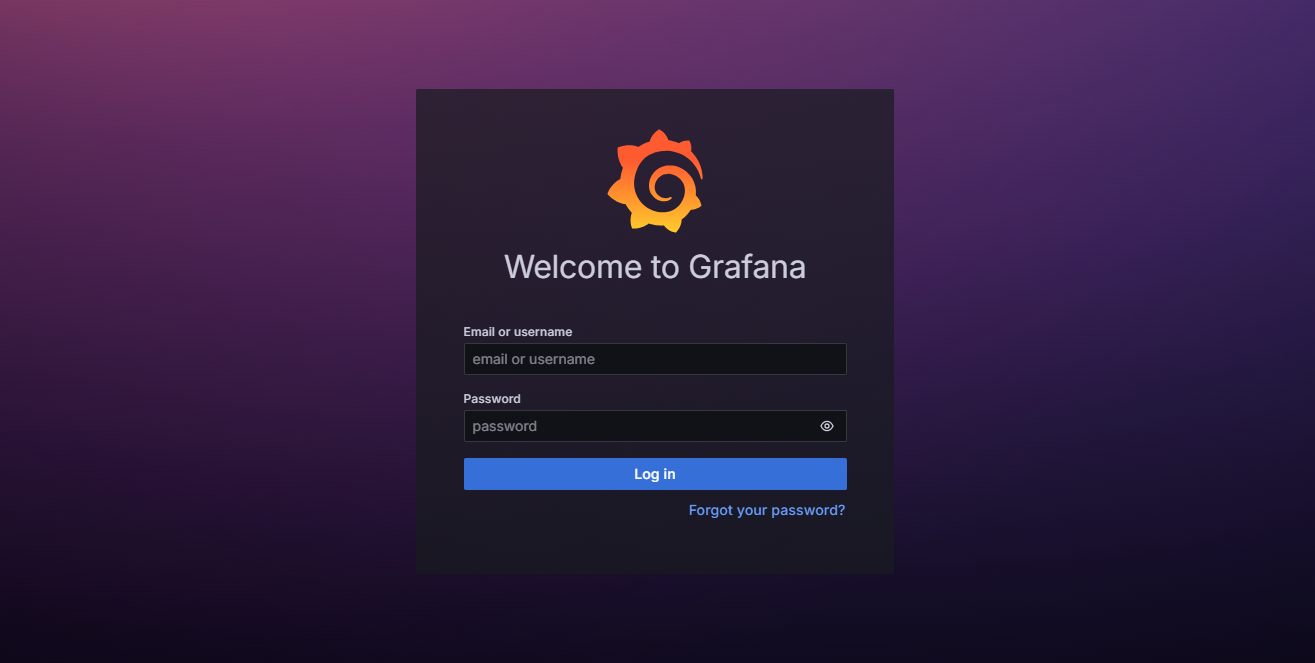
\includegraphics[width=0.7\linewidth]{login.png}
    \caption{Schermata di accesso al sistema}
\end{figure}
\noindent
In caso di credenziali errate, il sistema mostrerà un messaggio di errore, offrendo all'utente la possibilità di reimpostare le credenziali.
\begin{figure}[H]
    \centering
    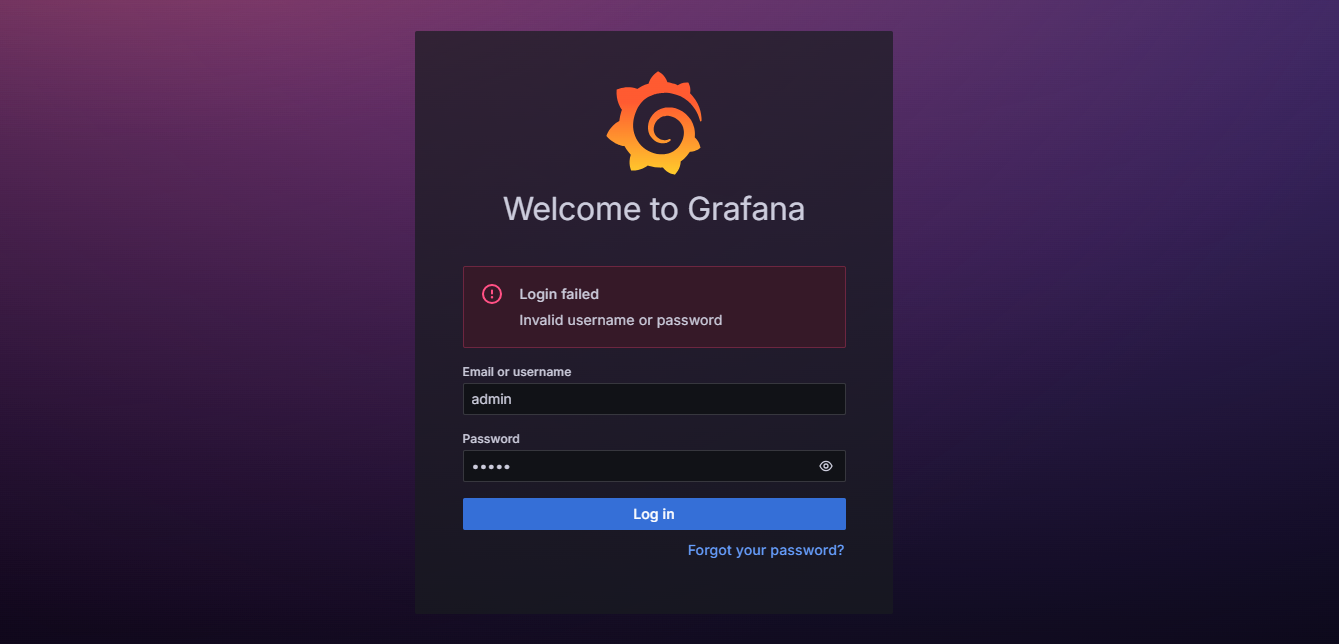
\includegraphics[width=0.7\linewidth]{error.png}
    \caption{Schermata di accesso in caso di messaggio di errore}
\end{figure}

\subsection{Dashboard}
La dashboard principale rappresenta il cruscotto di controllo del sistema ed è composta da due pannelli personalizzabili, che consentono la visualizzazione dei dati attraverso diverse modalità, tra cui una mappa interattiva con dei marker e una tabella riepilogativa.\\
Ogni pannello è progettato per presentare i dati in modo ottimale in base alla loro tipologia. In particolare, per le informazioni di natura geospaziale, viene utilizzata una mappa che mostra dei marker che rappresentano la posizione dei sensori, delle attività e dei messaggi pubblicitari, insieme ai relativi dettagli. All'interno della dashboard principale, è inoltre presente un pannello tabellare che fornisce un report dettagliato delle attività, aggregandole in base al numero di messaggi generati nell'ultimo mese. Questo consente di ottenere una panoramica chiara e strutturata sull'andamento del sistema.\\
Oltre alla dashboard principale, gli utenti autorizzati possono accedere alle dashboard specifiche degli utenti standard, ciascuna composta da un pannello dedicato alla visualizzazione della mappa, che include marker per ogni attività e si concentra sull'intero percorso svolto e su tutti i messaggi ricevuti dal singolo utente.\\
\begin{figure}[H]
    \centering
    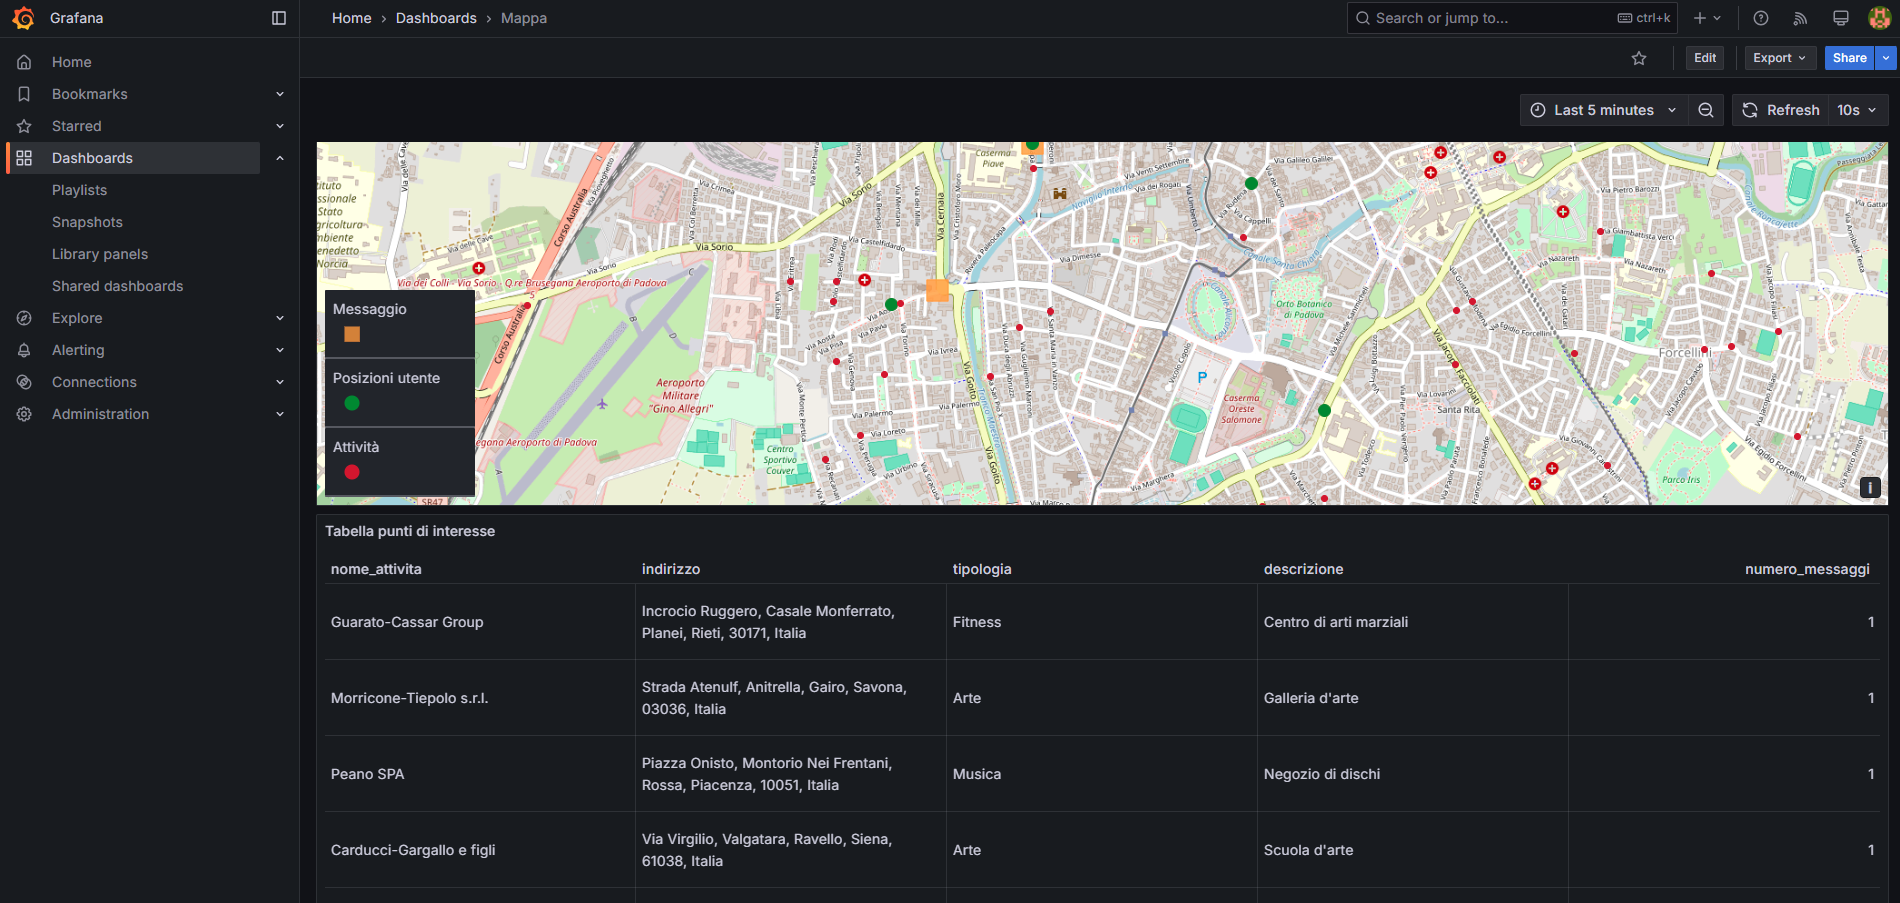
\includegraphics[width=1\linewidth]{dashboard.png}
    \caption{Dashboard principale}
\end{figure}

    \subsubsection{Barra degli strumenti} % pulsante edit mode da tenere?
    La barra degli strumenti, situata nella parte superiore della dashboard, offre una serie di opzioni aggiuntive tramite pulsanti e menù a tendina, che consentono di eseguire azioni specifiche e accedere a funzionalità aggiuntive in modo semplice e rapido.\\
    \begin{figure}[H]
    \centering
    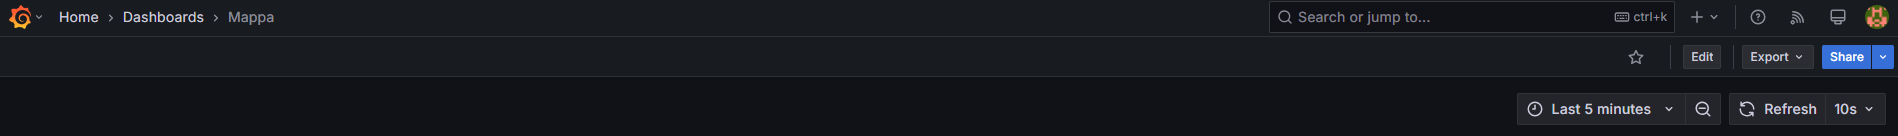
\includegraphics[width=1\linewidth]{barra.png}
    \caption{Barra degli strumenti}
    \end{figure}

    \paragraph{Pulsante profilo utente}
    Il pulsante del ``profilo utente" consente di accedere rapidamente alle impostazioni personali, dove è possibile visualizzare e modificare le informazioni del proprio account. Premendo il pulsante, viene visualizzato un menù a tendina con le seguenti opzioni:
    \begin{itemize}
        \item[-] \textbf{Profile}: permette di consultare e aggiornare le informazioni personali;
        \item[-] \textbf{Notification history}: consente di visualizzare la cronologia delle notifiche ricevute;
        \item[-] \textbf{Change password}: offre la possibilità di modificare la password dell'account;
        \item[-] \textbf{Sign out}: consente di effettuare il logout dal sistema.
    \end{itemize}
    \begin{figure}[H]
    \centering
    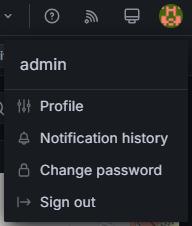
\includegraphics[width=0.25\linewidth]{profilo.png}
    \caption{Pulsante profilo utente}
    \end{figure}

    \paragraph{Barra di ricerca}
    La barra di ricerca consente agli utenti autorizzati di cercare e filtrare rapidamente le dashboard disponibili o di navigare all'interno del sistema. È possibile digitare il nome della dashboard o della pagina desiderata e premere ``Invio" per visualizzare i risultati corrispondenti.
    \begin{figure}[H]
    \centering
    
\includegraphics[width=0.6\linewidth]{ricerca.png}
    \caption{Barra di ricerca}
    \end{figure}

    \paragraph{Menù}
    Il menù, accessibile tramite l'icona di Grafana situata sulla barra degli strumenti, offre agli utenti autorizzati l'accesso a diverse funzionalità aggiuntive. Le opzioni disponibili sono le seguenti:
    \begin{itemize}
        \item[-] \textbf{Home}: consente di tornare alla homepage;
        \item[-] \textbf{Bookmarks}: permette di visualizzare i collegamenti salvati per un accesso rapido;
        \item[-] \textbf{Starred}: mostra l'elenco delle dashboard contrassegnate come preferite;
        \item[-] \textbf{Dashboards}: consente di accedere alla lista completa delle dashboard disponibili;
        \item[-] \textbf{Explore}: offre strumenti per esplorare i dati e analizzarli in tempo reale;
        \item[-] \textbf{Altering}: permette di visualizzare, gestire ed esportare le regole di allerta e le notifiche;
        \item[-] \textbf{Connections}: consente di gestire le connessioni a database e fonti dati esterne;
        \item[-] \textbf{Administration}: fornisce accesso alle impostazioni avanzate e alla gestione degli utenti e dei permessi.
    \end{itemize}
    \begin{figure}[H]
    \centering
    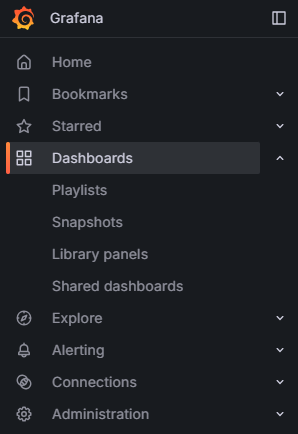
\includegraphics[width=0.35\linewidth]{menu.png}
    \caption{Menù}
    \end{figure}

    \paragraph{Breadcrumb}
    La breadcrumb mostra il percorso di navigazione dell'utente autorizzato e indica la sua posizione corrente all'interno del sistema attraverso una serie di link. Questi link consentono di navigare facilmente tra le sezioni, permettendo all'utente di tornare rapidamente alle pagine precedenti.
    \begin{figure}[H]
    \centering
    
\includegraphics[width=0.35\linewidth]{breadcrumb.png}
    \caption{Breadcrumb}
    \end{figure}

    \paragraph{Pulsante Mark as favorite}
    Il pulsante ``Mark as favorite" consente di aggiungere una dashboard all'elenco delle preferite, facilitandone l'accesso rapido.
    \begin{figure}[H]
    \centering
    
\includegraphics[width=0.18\linewidth]{favorite.png}
    \caption{Pulsante ``Mark as favorite"}
    \end{figure}

    \paragraph{Pulsante Export}
    Il pulsante ``Export" consente di esportare una dashboard in formato JSON.
    \begin{figure}[H]
    \centering
    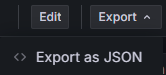
\includegraphics[width=0.2\linewidth]{export.png}
    \caption{Pulsante ``Export"}
    \end{figure}

    \paragraph{Pulsante Share}
    Il pulsante ``Share", consente di condividere la dashboard attualmente visualizzata. Cliccando sulla freccia rivolta verso il basso accanto al pulsante, si apre un menù con le seguenti opzioni:
    \begin{itemize}
        \item[-] \textbf{Share internally}: per condividere la dashboard con altri utenti all'interno dell'organizzazione, mantenendo il controllo sugli accessi e sui permessi;
        \item[-] \textbf{Share externally}: per rendere la dashboard accessibile pubblicamente, generando un link che chiunque può utilizzare per visualizzare la dashboard in modalità di sola lettura;
        \item[-] \textbf{Share snapshot}: per creare uno snapshot della dashboard da condividere. Questo metodo consente di condividere lo stato attuale della dashboard, rimuovendo dati sensibili come query e link ai pannelli.
    \end{itemize}
    \begin{figure}[H]
    \centering
    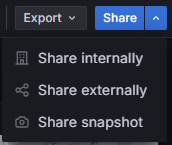
\includegraphics[width=0.25\linewidth]{share.png}
    \caption{Pulsante ``Share"}
    \end{figure}

    \paragraph{Time settings}
    Il menù a tendina ``Time settings" permette all'utente di selezionare l'intervallo temporale desiderato per la visualizzazione dei dati. La dashboard offre una serie di intervalli predefiniti e consente all'utente di personalizzarli secondo le proprie necessità. Le aggregazioni delle misurazioni e le operazioni sui dati vengono applicate in base all'intervallo temporale selezionato, garantendo un'analisi accurata e contestualizzata delle informazioni.
    \begin{figure}[H]
    \centering
    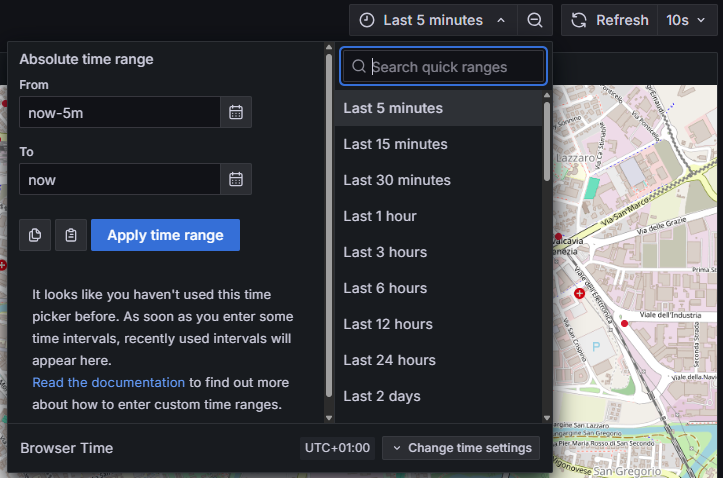
\includegraphics[width=0.7\linewidth]{time.png}
    \caption{Menù ``Time settings"}
    \end{figure}

    \paragraph{Pulsante Zoom out}
    Il pulsante ``Zoom out" consente di estendere l'intervallo temporale visualizzato nei grafici, permettendo di analizzare periodi più ampi di dati. Cliccando su questo pulsante, la visualizzazione si adatta automaticamente per mostrare un intervallo temporale più esteso, secondo gli intervalli predefiniti.
    \begin{figure}[H]
    \centering
    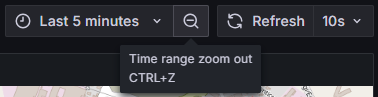
\includegraphics[width=0.45\linewidth]{zoomout.png}
    \caption{Pulsante ``Zoom out"}
    \end{figure}
    
    \paragraph{Pulsante Refresh}
    Il pulsante ``Refresh" consente all'utente di aggiornare la dashboard attualmente visualizzata per ottenere i dati più recenti. Cliccando sulla freccia accanto al pulsante, si apre un menù a tendina che offre diverse opzioni per la frequenza di aggiornamento:
    \begin{itemize}
        \item[-] \textbf{Off}: disattiva l'aggiornamento automatico;
        \item[-] \textbf{Auto}: aggiorna la dashboard a intervalli dinamici, determinati dalla durata dell'intervallo temporale visualizzato e dalla larghezza della finestra del browser;
        \item[-] \textbf{Intervalli predefiniti}: permettono di impostare un aggiornamento automatico a intervalli specifici (ad esempio, 5s, 10s, 30s, 1m, ecc.).
    \end{itemize}
    Di default, le dashboard del sistema sono configurate per aggiornarsi automaticamente ogni 10 secondi. Questa impostazione può essere modificata in base alle esigenze dell'utente autorizzato.
    \begin{figure}[H]
    \centering
    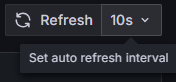
\includegraphics[width=0.25\linewidth]{refresh.png}
    \caption{Pulsante ``Refresh"}
    \end{figure}


    \subsubsection{Pannelli}
    I pannelli costituiscono la componente principale della dashboard, presentando i dati in modo interattivo. Ogni pannello è un widget progettato per visualizzare un insieme specifico di dati, utilizzando una forma appropriata in base alla loro tipologia. Nel contesto del sistema in questione, i pannelli includono una mappa generale, delle mappe specifiche per utenti e una tabella riepilogativa dei punti di interesse.\\
    Gli elementi presenti nei pannelli sono:
    \begin{itemize}
        \item[-] Nome del pannello;
        \item[-] Legenda (se presente);
        \item[-] Menù opzioni del pannello;
        \item[-] Visualizzazione dei dati.
    \end{itemize}

    \paragraph{Legenda}
    La legenda è una sezione del pannello che fornisce la chiave di lettura dei dati visualizzati. È utile per comprendere il significato dei colori e delle forme utilizzate nel pannello. Viene impiegata solamente nei pannelli che contengono una mappa.
    \begin{figure}[H]
    \centering
    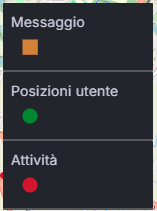
\includegraphics[width=0.25\linewidth]{legenda.png}
    \caption{Legenda}
    \end{figure}

    \paragraph{Menù Opzioni}
    Cliccando sull'icona con tre puntini verticali nell'angolo in alto a destra di un pannello in Grafana, è possibile accedere a diverse funzionalità, tra cui la visualizzazione a schermo intero, la condivisione o l'esportazione del pannello, l'esplorazione delle query per un'analisi più approfondita, l'ispezione dei dati visualizzati, l'accesso a opzioni aggiuntive e la modifica del pannello per personalizzarne le impostazioni.
    \begin{figure}[H]
    \centering
    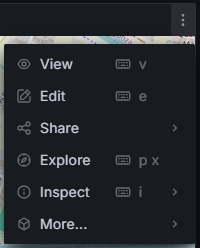
\includegraphics[width=0.25\linewidth]{opzioni.png}
    \caption{Opzioni del pannello}
    \end{figure}

\subsection{Struttura e funzionalità dei pannelli}
Questa sezione descrive nel dettaglio i pannelli principali che compongono le dashboard del sistema, fornendo una panoramica delle funzionalità e delle informazioni visualizzate. In particolare, sono disponibili tre tipi di pannelli, descritti di seguito.

    \subsubsection{Mappa generale}
    La mappa generale presenta una visualizzazione globale dei dati geospaziali, utilizzando dei marker distinti per rappresentare diverse entità ed attività:
    \begin{itemize}
        \item[-] \textbf{Punti di interesse}: indicati da dei marker rossi immobili, evidenziano le attività che offrono dei servizi;
        \item[-] \textbf{Sensori}: rappresentati da dei marker verdi in movimento, seguono gli spostamenti degli utenti sulla mappa e forniscono dati in tempo reale sulla loro ultima posizione;
        \item[-] \textbf{Messaggi pubblicitari}: mostrati come quadrati arancioni, indicano l'ultimo messaggio pubblicitario generato per ciascun utente. Questi sono visibili solo se l'utente si trova all'interno dell'area di influenza dell'attività correlata.
    \end{itemize}
    La mappa include una leggenda che associa colori e forme alle diverse categorie di dati per facilitarne l'interpretazione. Inoltre, è possibile navigare sulla mappa con il mouse, mentre lo zoom può essere regolato utilizzando la rotella del mouse o tramite i pulsanti ``+" e ``-" situati sotto il nome del pannello.
    \begin{figure}[H]
    \centering
    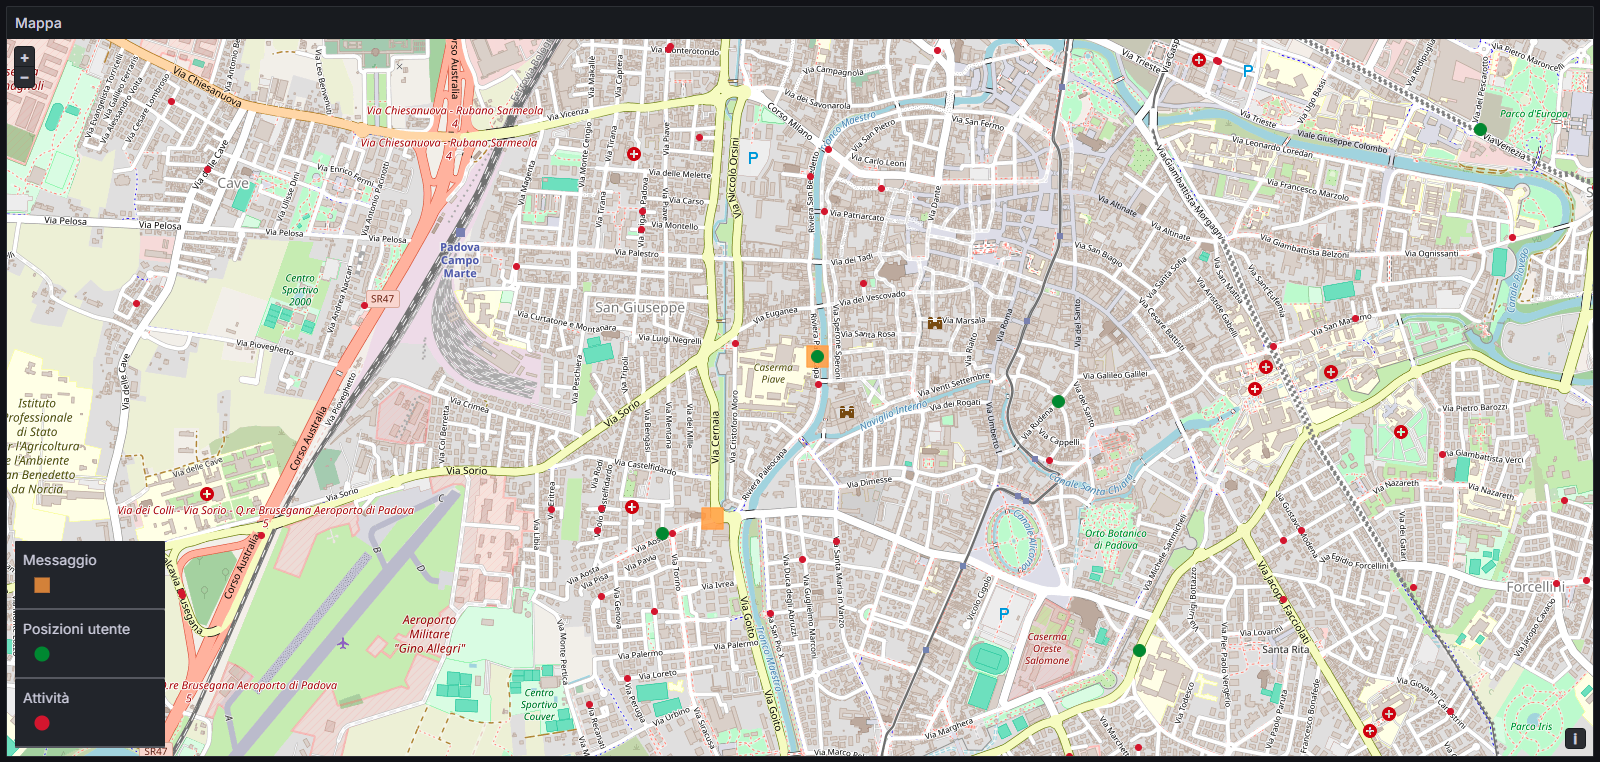
\includegraphics[width=1\linewidth]{mappa.png}
    \caption{Pannello mappa generale}
    \end{figure}
    
    \subsubsection{Tabella attività}
    La tabella mostra una le attività raggruppate per numero di messaggi generati nel mese corrente. I campi visualizzati includono: nome dell'attività, indirizzo, numero di messaggi generati e tipologia. Questo pannello è presente insieme alla mappa generale nella dashboard principale.
    \begin{figure}[H]
    \centering
    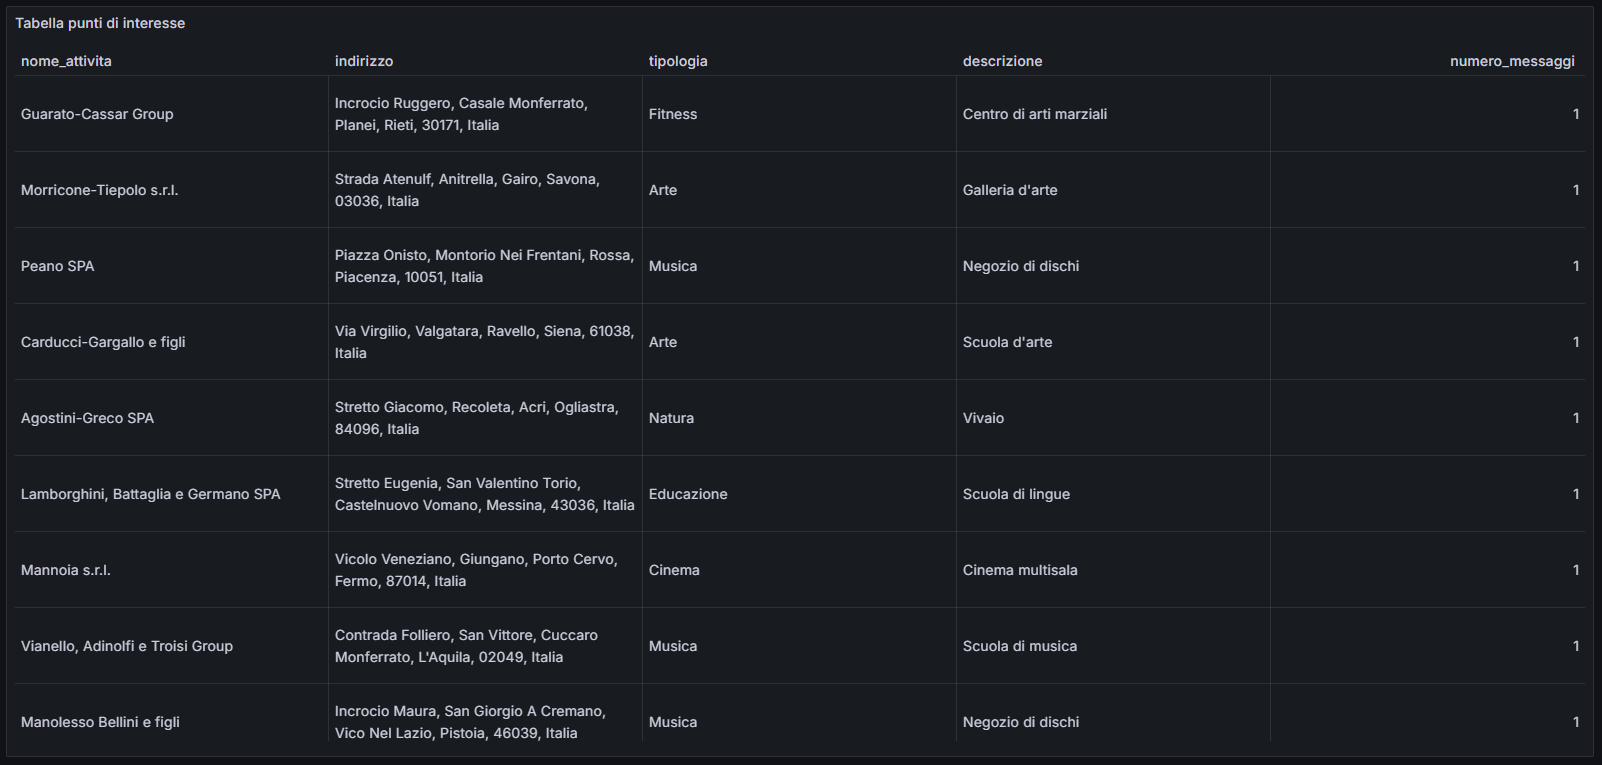
\includegraphics[width=1\linewidth]{tabella.png}
    \caption{Pannello tabella attività}
    \end{figure}
    
    \subsubsection{Mappa specifica}
    La mappa specifica presenta una visualizzazione globale dei dati geospaziali relativi ad un singolo utente, utilizzando dei marker distinti per rappresentare diverse entità e attività:
    \begin{itemize}
        \item[-] \textbf{Punti di interesse}: indicati da dei marker rossi immobili, evidenziano le attività che offrono dei servizi;
        \item[-] \textbf{Percorso dell'utente}: rappresentato da dei marker viola che tracciano tutte le posizioni percorse dal singolo utente. La prima e l'ultima posizione del percorso sono evidenziate da un contorno verde;
        \item[-] \textbf{Messaggi pubblicitari}: mostrati come quadrati arancioni, indicano tutti i messaggi pubblicitari ricevuti dall'utente, posizionati esattamente nel punto in cui sono stati ricevuti.
    \end{itemize}
    La mappa include una leggenda che facilita l'interpretazione dei marker. Inoltre, è possibile navigare sulla mappa con il mouse, mentre lo zoom può essere regolato utilizzando la rotella del mouse o tramite i pulsanti ``+" e ``-" situati sotto il nome del pannello.
    \begin{figure}[H]
    \centering
    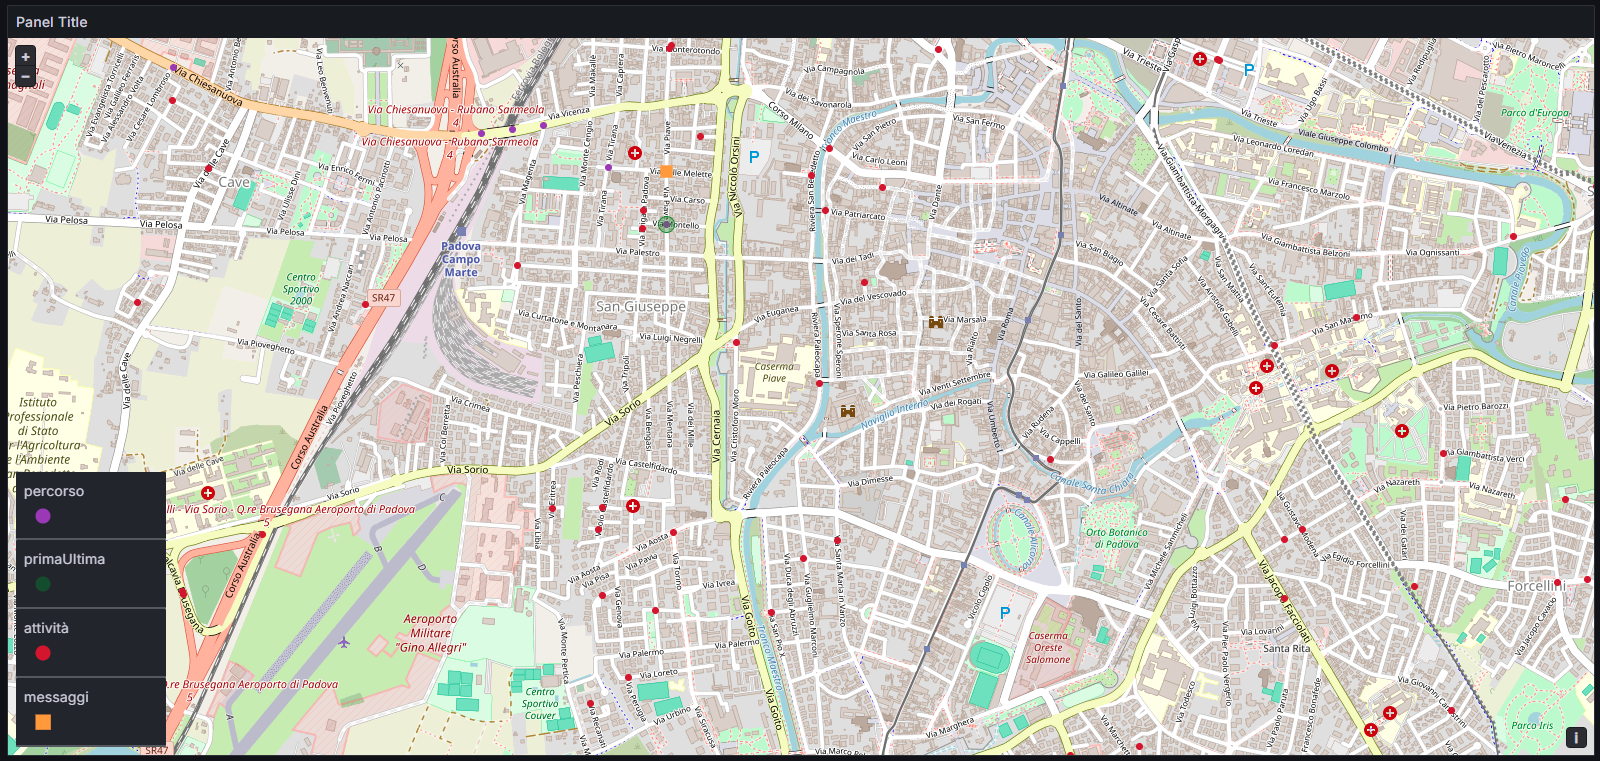
\includegraphics[width=1\linewidth]{mappaspec.png}
    \caption{Pannello mappa specifica per singolo utente}
    \end{figure}

    \subsubsection{Tabella attività}
    La tabella mostra una le attività raggruppate per numero di messaggi generati nel mese corrente. I campi visualizzati includono: nome dell'attività, indirizzo, descrizione, numero di messaggi generati e tipologia. Questo pannello è presente insieme alla mappa generale nella dashboard principale.
    \begin{figure}[H]
    \centering
    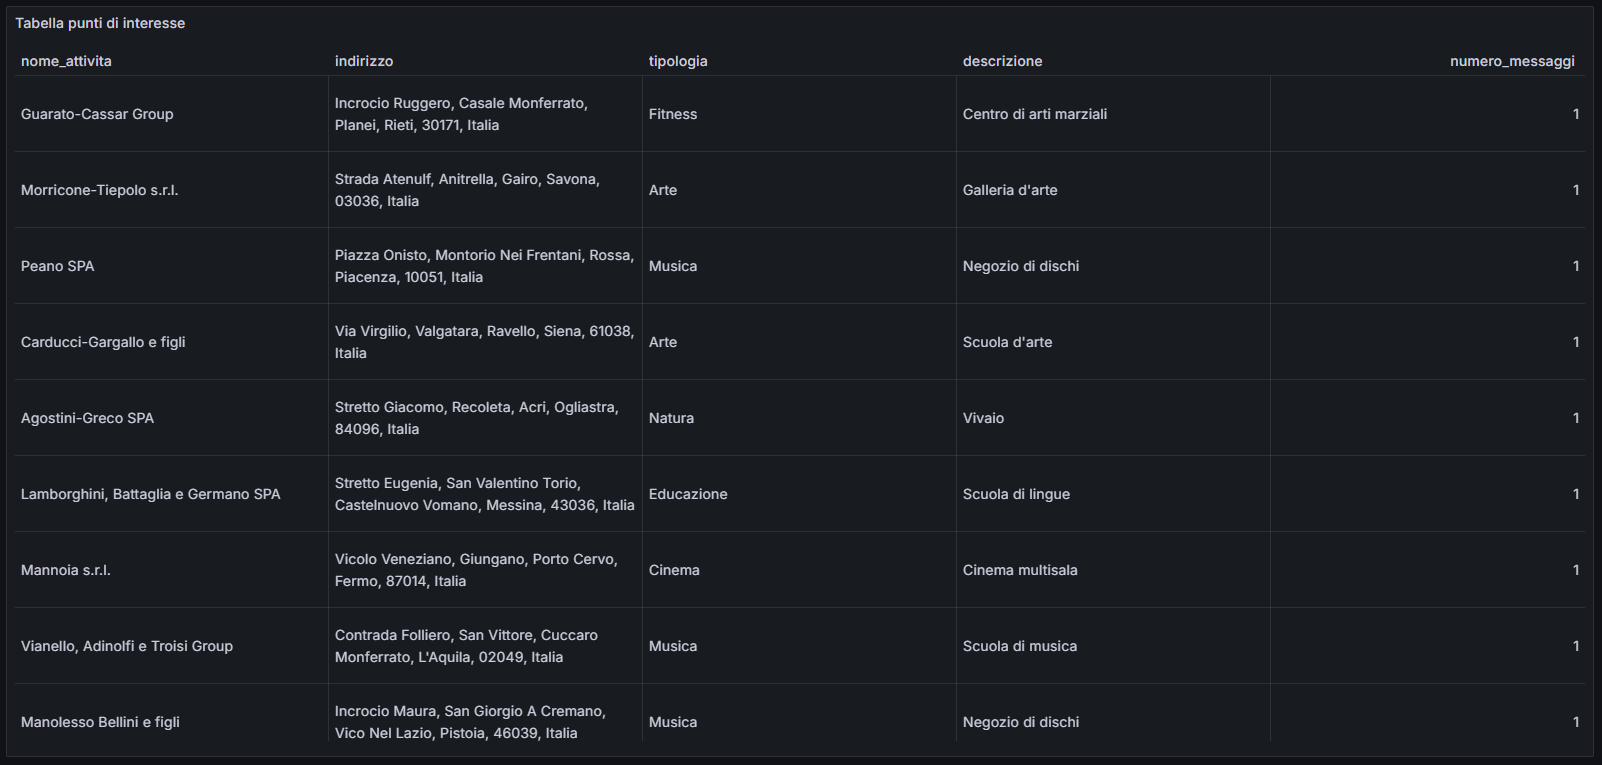
\includegraphics[width=1\linewidth]{tabella.png}
    \caption{Pannello tabella attività}
    \end{figure}

    \subsubsection{Anagrafica Utente}
    Il pannello mostra i dati anagrafici di un determinato utente presente nel sistema. La tabella visualizzata include il nome, il cognome, l'indirizzo email, il genere e la data di nascita. Inoltre, vengono riportate alcune informazioni utili per la personalizzazione delle campagne pubblicitarie, come lo stato civile e gli interessi principali. Queste informazioni sono accessibili direttamente dalla mappa specifica dell'utente e possono essere sfruttate per analisi statistiche e strategie di marketing mirate.  
    \begin{figure}[H]
    \centering
    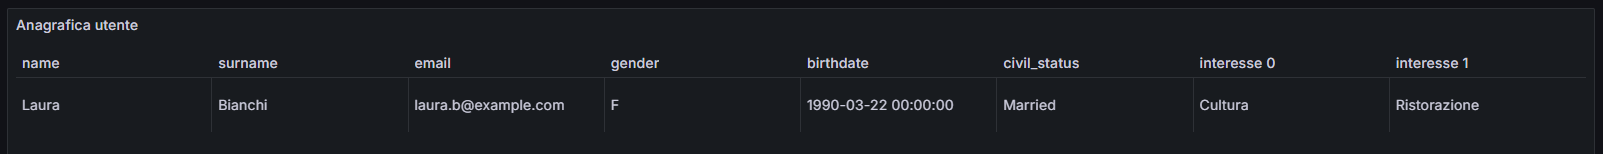
\includegraphics[width=1\linewidth]{anagrafica.png}
    \caption{Pannello anagrafica utente}
    \end{figure}



\subsection{Profilo Utente}
La pagina del profilo utente è accessibile cliccando sull'icona dell'utente situata nell'angolo in alto a destra della barra degli strumenti. Da qui, gli utenti autorizzati possono visualizzare e modificare le proprie informazioni personali, oltre ad accedere alle preferenze per apportare eventuali modifiche.\\
La schermata del profilo utente è suddivisa in tre schede principali:  
\begin{itemize}  
    \item[-] Profile; 
    \item[-] Notification history; 
    \item[-] Change password.  
\end{itemize}
    
    \subsubsection{Profile}
    La schermata dedicata al profilo permette di visualizzare e modificare le proprie informazioni personali. In particolare, è possibile aggiornare il nome, l'email e lo username. Dopo aver apportato le modifiche desiderate, è possibile salvarle cliccando sul pulsante ``Save".\\
    Sono inoltre disponibili tre sottosezioni aggiuntive:
    \begin{itemize}
        \item[-] Preferences;
        \item[-] Organizations;
        \item[-] Sessions.
    \end{itemize}
    \begin{figure}[H]
    \centering
    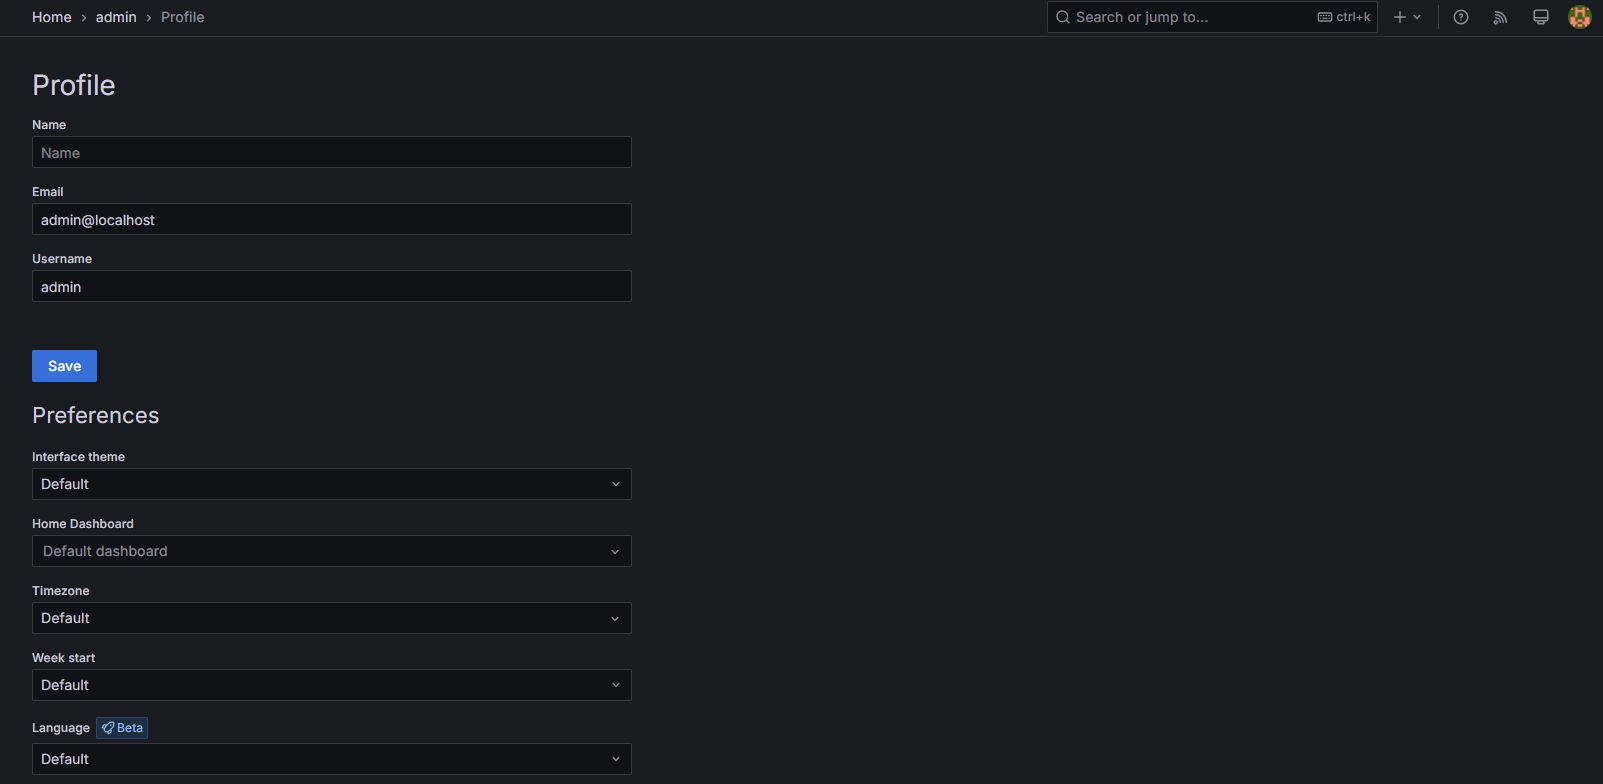
\includegraphics[width=1\linewidth]{profile.png}
    \caption{Schermata del profilo utente}
    \end{figure}

    \paragraph{Preferences}
    La seguente sezione consente di modificare le proprie preferenze:  
    \begin{itemize}  
        \item[-] Tema dell'interfaccia;  
        \item[-] Dashboard predefinita (Home dashboard);  
        \item[-] Fuso orario;  
        \item[-] Inizio della settimana;  
        \item[-] Lingua.  
    \end{itemize}  
    Una volta effettuate le modifiche desiderate, è possibile confermarle cliccando sul pulsante ``Save". 
    
    \paragraph{Organizations}
    La seguente sezione consente di visualizzare le organizzazioni a cui l'utente appartiene. Per ogni organizzazione, è possibile visualizzare il nome e il ruolo dell'utente al suo interno.  
    
    \paragraph{Sessions}
    La seguente sezione consente di visualizzare le sessioni attive dell'utente. Per ciascuna sessione, è possibile visualizzare la data e l'ora dell'ultimo accesso, l'indirizzo IP, nonché il browser e il sistema operativo utilizzati. Attraverso un pulsante dedicato, è possibile terminare la sessione desiderata.

    \subsubsection{Notification history}
    Questa schermata consente di visualizzare la cronologia delle notifiche relative a errori o avvertenze. Per ciascuna notifica, è possibile visualizzare la data e l'ora, il tipo di notifica e, se presente, il messaggio corrispondente. È possibile selezionare una o più notifiche e, cliccando sul pulsante ``Dismiss Notifications", eliminarle. Una volta cancellate, le notifiche non saranno più recuperabili.
    \begin{figure}[H]
    \centering
    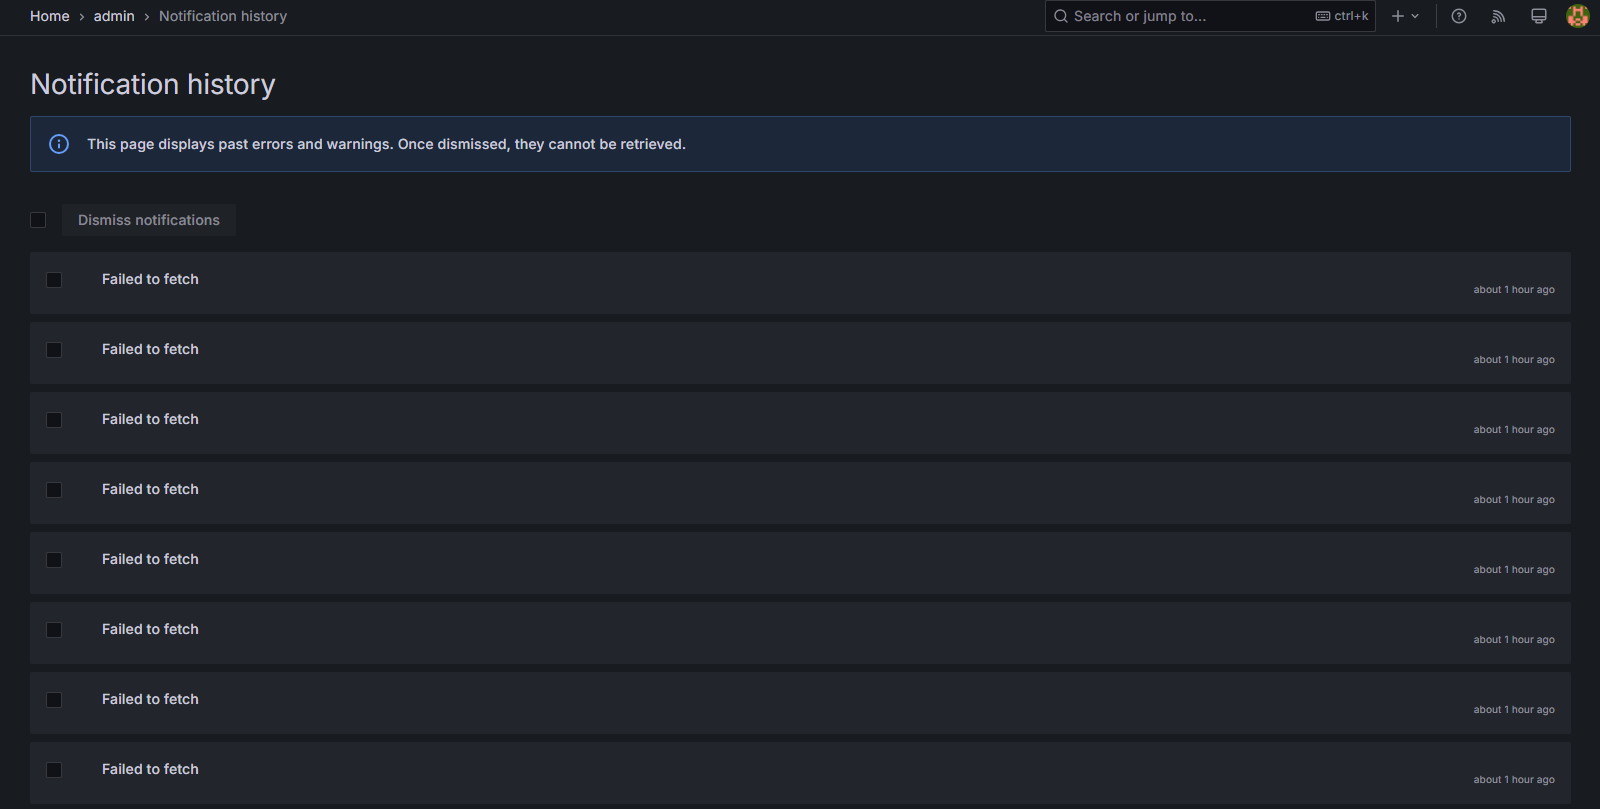
\includegraphics[width=1\linewidth]{notification.png}
    \caption{Schermata cronologia delle notifiche}
    \end{figure}

    \subsubsection{Change password}
    Questa schermata consente di modificare la propria password. Per effettuare la modifica, è necessario inserire la password corrente, la nuova password e confermare quest'ultima. Una volta inserite le informazioni richieste, è possibile confermare le modifiche cliccando sul pulsante ``Change Password", oppure annullare le modifiche cliccando su ``Cancel".\\
    Cliccando sull'icona a forma di occhio, è possibile visualizzare la password inserita. Cliccando nuovamente sull'icona, la password verrà nascosta nuovamente.
    \begin{figure}[H]
    \centering
    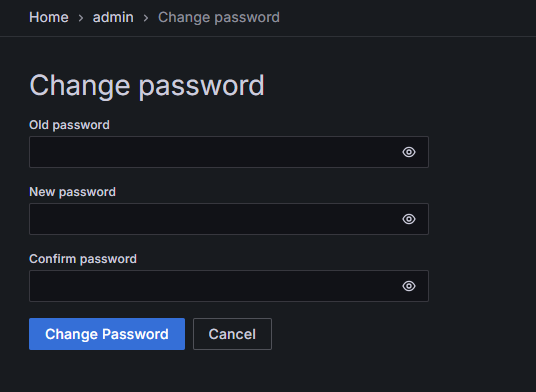
\includegraphics[width=0.5\linewidth]{password.png}
    \caption{Schermata cambio della password}
    \end{figure}

\newpage

\section{Supporto Tecnico}
\label{sec:supporto}
Per ricevere assistenza su problemi tecnici, difficoltà nell'installazione o dubbi relativi all'utilizzo del sistema, è possibile contattare il team di supporto all'indirizzo email: \texttt{sevenbits.swe.unipd@gmail.com}.\\
Il team si impegna a fornire una risposta tempestiva con le informazioni necessarie per risolvere eventuali problematiche.\\
Nel messaggio di richiesta supporto, è consigliato includere una descrizione chiara del problema, eventuali messaggi di errore ricevuti, la data e l'ora in cui è stato riscontrato il malfunzionamento, e possibilmente degli screenshot o altri dettagli che possano tornare utili per la risoluzione.



%% Codice per Immagini %%

%\begin{figure}[ht]
%    \centering
%    \includegraphics[width=0.5\linewidth]{NomeImmagine.png}
%    \caption{TestoCaption}
%    \label{LabelImmagine}
%\end{figure}


%% Codice per Tabelle %%

%\begin{center}
%\renewcommand{\arraystretch}{1.5}
%\begin{longtable}
%{|>{\centering\arraybackslash}m{2.7cm}|>       {\centering\arraybackslash}m{2.7cm}|>{\centering\arraybackslash}m{2.1cm}|}
%\hline
%\textbf{} & \textbf{} & \textbf{}\\
%\endhead
%\hline
%\hline
%\caption{Requisiti$_G$ funzionali}
%\end{longtable}
%\end{center}

\end{justify}
\end{document}